\documentclass[12pt,a4paper]{article}
\usepackage[T1,T2A]{fontenc}
\usepackage[utf8]{inputenc}
\usepackage[english,russian]{babel}
\usepackage{amsmath}
\usepackage{graphicx}
\graphicspath{{pictures/}}
\DeclareGraphicsExtensions{.pdf,.png,.jpg}

\title{\LaTeX}  
\date{}  
\author{Артём Алексеев}
\setlength{\parskip}{6pt}
\setlength{\parindent}{0ex}

\begin{document}

\section{Интегралы}
\subsection{Таблица интегралов}

\begin{minipage}{0.4\textwidth}
\begin{flushleft}
$ \int{0dx} = C $ 

$ \int{dx} = x + C $ 

$ \int{x^n dx} = \frac{x^{n+1}}{n+1} + C $ 

$ \int{\frac{dx}{x}} = \ln{|x|} + C $ 

$ \int{a^x dx} = \frac{a^x}{\ln{a}} + C $ 

$ \int{e^x dx} = e^x + C $ 

$ \int{\cos{x}dx} = \sin{x} + C $ 

$ \int{\sin{x}dx} = -\cos{x} + C $
\end{flushleft}
\end{minipage}
\hfill
\begin{minipage}{0.5\textwidth}
\begin{flushleft}
$ \int{\frac{dx}{\sin^2{x}}} = -ctg{x} + C $ 

$ \int{\frac{dx}{\cos^2{x}}} = \tg{x} + C $ 

$ \int{\frac{dx}{x^2+a^2}} = \frac{1}{a} \arctan \frac{x}{a} + C $ 

$ \int{\frac{dx}{\sqrt{a^2-x^2}}} = \arcsin{x/a} + C $ 

$ \int{\frac{dx}{a^2-x^2}}=\frac{1}{2a}\ln{|\frac{a+x}{a-x}|} + C, x \neq a $ 

$ \int{\frac{dx}{\sqrt[]{x^2 \pm a^2}}} = \ln{|x + \sqrt[]{x^2 \pm a^2}|} + C $
\end{flushleft}
\end{minipage}

\subsection{Свойства интегралов}

1) $ (\int{f(x)dx})' = f(x) $ 

2) $ \int{d(f(x)} = f(x) + C $ 

3) $ \int{k f(x)dx} = k \int{f(x)dx)} $ 

4) $ \int{(f(x) \pm g(x))dx} = \int{f(x)dx} \pm \int{g(x)dx}$

\subsection{Метод замены переменной}
\subsubsection{Подведение функции под знак дифференциала}

Пример 1: 

$ \int{\sin(3x + 1)dx} $ 

Подводим $ (3x+1) $ под знак диференциала 

$ \int{\sin(3x + 1)dx} = \frac{1}{3}\int{sin(3x+1}d(3x+1) $ 

По таблице $ \int{sin(x)dx} = -cos(x) + C $ 

$ \frac{1}{3}\int{sin(3x+1)d(3x+1)} = -\frac{1}{3}cos(3x+1) + C $

Пример 2: 

$ \int{\frac{dx}{5 - 2x}} = -\frac{1}{2}\int{\frac{d(5-2x)}{5 - 2x}}
= -\frac{1}{2}ln|5-2x|+C $

\subsubsection{Замена переменной}
Пример 1: 

$ \int{\sin(3x + 1)dx} $ 

$ t = 3x + 1 $ 

$ dx = \frac{dt}{3} $ 

$ \int{\sin(3x + 1)dx} = \frac{1}{3}\int{sin(t)dt} = -\frac{1}{3}cos(t) + C = -\frac{1}{3}cos(3x+1) + C $ 

\subsection{Метод интегрирования по частям}
\subsubsection{Интегралы от логарифмов}
\textbf{Общее правило}: за u всегда обозначается логарифм

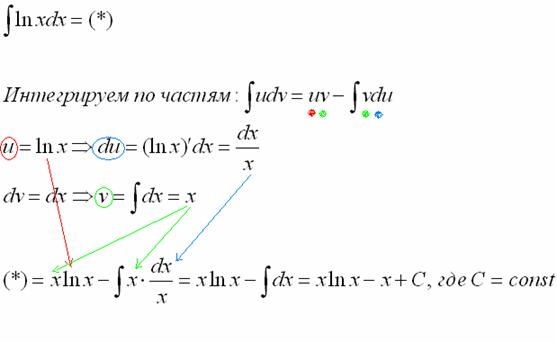
\includegraphics[width=\linewidth]{partial_integration}

\subsubsection{Интегралы от экспоненты, умноженной на многочлен}

\textbf{Общее правило}: за u всегда обозначается многочлен

Пример:

$\int{(x-2)e^{2x}dx} = (*) $

$ u = x-2 => du = (x-2)'dx = dx $

$ dv = e^{2x}dx => v = \int{e^{2x}dx} = \frac{1}{2}e^{2x} $

$ \int{vdu} = uv - \int{vdu} $

$ (*) = \frac{(x-2)e^{2x}}{2} - \frac{1}{2}\int{e^{2x}}dx = \frac{(x-2)e^{2x}}{2} - \frac{1}{2}* \frac{1}{2}e^{2x} + C 
= \frac{(x-2)e^{2x}}{2} - \frac{e^{2x}}{4} + C $

\subsubsection{Интегралы от тригонометрических функций, умноженных на многочлен}

\textbf{Общее правило}: за u всегда обозначается многочлен

$ \int{x cos6xdx} = (*) $ 

$ u = x => du = dx $

$ dv = cos6xdx => v = \int{cos6xdx} = \frac{1}{6}sin6x $

$ \int{vdu} = uv - \int{vdu} $

$ (*) = \frac{1}{6}xdx - frac{1}{6}\int{sin6xdx} 
= \frac{1}{6}xsin6x-\frac{1}{6}(-\frac{1}{6}cos6x) 
= \frac{1}{6}xsin6x+\frac{1}{36}cos6x+C $

\subsubsection{Интегралы от обратных тригонометрических функций. Интегралы от обратных тригонометрических функций, умноженных на многочлен}

\textbf{Общее правило}: за u всегда обозначается обратная тригонометрическая функция

$ \int{arctg2xdx} = (*) $ 

$ u = arctg2x => du = \frac{1}{1+(2x)^2} * (2x)'dx = \frac{2dx}{1+4x^2} $

$ dv = dx => v = x $

$ \int{vdu} = uv - \int{vdu} $

$ (*) =	xarctg2x - 2 \int frac{xdx}{1+4x^2} 
= xarctg2x - \frac{1}{4}\int\frac{d(1+4x^2}{1+4x^2}
= xarctg2x - \frac{1}{4}ln(1+4x^2) + C $

\subsection{Метод неопределенных коэффициентов}
Для интегрирования рациональной функции $\frac{P(x)}{Q(x)}$ используется Алгоритм:

1. Если дробь неправильная (старшая степень числителя больше или равна старшей степени знаменателя), преобразовать ее в правильную, выделив целое выражение; 

2. Разложить знаменатель на произведение одночленов и/или несократимых квадратичных выражений; 

3. Разложить рациональную дробь на простейшие дроби, используя метод неопределенных коэффициентов; 

4. Вычислить интегралы от простейших дробей. 

Пример: 

$ \int{\frac{x^2-19x+6}{(x-1)(x^2+5x+6)}dx} $ 

Старшая степени числителя - 2, знаменателя - 3, значит дробь правильная 

$ \int{\frac{x^2-19x+6}{(x-1)(x+2)(x+3)}dx} $ 

$ \frac{x^2-19x+6}{(x-1)(x+2)(x+3)}=\frac{A}{x-1}+\frac{B}{x+2}+\frac{C}{x+3} $ 

$ \frac{x^2-19x+6}{(x-1)(x+2)(x+3)}=\frac{A(x+2)(x+3)+B(x-1)(x+3)+C(x-1)(x+2)}{(x-1)(x+2)(x+3)} $ 

$ x^2-19x+6=A(x+2)(x+3)+B(x-1)(x+3)+C(x-1)(x+2) $ 

$ x^2-19x+6=A(x^2+5x+6)+B(x^2+2x-3)+C(x^2+x-2) $ 

Если бы в левой части не было $x^2$, то представим что он равен $0*x^2$. 

Теперь все коэффициенты при степенях выписываем в соответствующие уравнения в систему уравнений. 

$\begin{cases}
A+B+C=1 \\
5A+2B+C=-19 \\
6A-3B-2C=6
\end{cases}$

$\begin{cases}
C=1-A-B \\
5A+2B+1-A-B=-19 \\
6A-3B-2(1-A-B)=6
\end{cases}$

$\begin{cases}
C=1-A-B \\
4A+B=-20 \\
8A-B=8
\end{cases}$

$ 12A=-12 $ 

$ A=-1; B=-16; C=18 $ 

Возвращаемся к интегалу 

$ \frac{x^2-19x+6}{(x-1)(x+2)(x+3)}=\frac{-1}{x-1}+\frac{-16}{x+2}+\frac{18}{x+3} $ 

$ \int{(-\frac{1}{x-1}-\frac{16}{x+2}+\frac{18}{x+3})dx}= $ 

$ =-\int{\frac{dx}{x-1}}-16\int{\frac{dx}{x+2}}+18\int{\frac{dx}{x+3}}= $ 

$ =-\ln|x-1|-16\ln|x+2|+18\ln|x+3|+C $ 

\end{document}
